\chapter{MC-SBD-STM on experimental data}
This chapter aims to demonstrate the application of the algorithm to real experimental data. We first elaborate the layers of complexity posed by real experimental data compared to the synthetic data. We then address the additional complexity by introducing a preprocessing pipeline that removes some common experimental artifacts and standardizes the experimental data condition before we apply the algorithm. Lastly, we applied the whole workflow to four different material systems. The results from these algorithm runs not only showcased the success and limitations of the algorithm, but also offered an opportunity to glance into the potential novel physics the method uncovers. 

\section{additional complexity in experimental data}
The phase space analysis in the last section showed the algorithm can worth robustly in vast regime of synthetic datasets. However, despite the effort we made to generate experiment-informed synthetic data, the real data might deviate from the synthetic data. For a practical application of this algorithm, it is essential to have the discussion around the complexities created by these deviations, with the focus on whether they will be a failure mode to the algorithm. We then created a pipeline that both addresses these failure modes and standardize the input dataset.

%todo: citation needed
While achieving low noise level in \ac{STM} is an important topic on its own \cite{geAchievingLowNoise2019}, the algorithm is robust against noise randomly distributed in space and time. The failure mode of the algorithm lies in any features that are structured but unwanted or non-intrinsic. There are three sources of these abnormality in \ac{STM} measurements: The sample surface getting contaminated, the tip being unstable, and an imperfect scanning environment. We will discuss the distinct complexities introduced by these three sources and how we mitigate each of them.  

Surface contamination introduces additional atoms or molecules that are non-intrinsic on the surface. It is unfavorable as it normally introduces non-repetitive features on the surface, and should be mitigated preferably by scanning on a cleaner area. However, if a completely clean surface is not accessible, minor contamination features can be suppressed by applying a truncated Gaussian mask; this mask is also used to perform the defect masking in standard STM-QPI analysis, which will be elaborated when introducing the preprocessing pipeline.

The operational environment of STM affects the noise level of the measurement; a potential failure mode of the algorithm comes from structured noise caused by temporal variation of the overall operational noise. For example, a grid spectroscopy measurement spans several days, and could experience different acoustic and vibrational noise levels over time, and the resulting grid map will have a noise pattern that varies across the image. A grid map acquired over a span of three days is shown in panel a) of Figure \ref{fig:periodic_noise}, with the variation in noise along the slow scan direction plotted at the bottom. Three distinct high–low noise cycles are observed, corresponding to day–night transitions during the measurement period. To mitigate this structured, periodic noise, we apply a variance-leveling procedure by adding noise to the low-noise regions, matching their variance to that of the high-noise regions. The resulting processed image is shown in panel b). While this approach increases the overall noise level, it effectively removes the structured noise, thereby enhancing the reliability of the outputs—though it may slightly reduce the success rate of the algorithm due to the higher uniform noise floor. This trade-off is acceptable for some datasets but can lead to complete algorithmic failure in others; the PtSn$\textsubscript{4}$ dataset shown in Figure. \ref{fig:periodic_noise} falls into the latter category and will be elaborated in section 7.6. 



\begin{figure}
	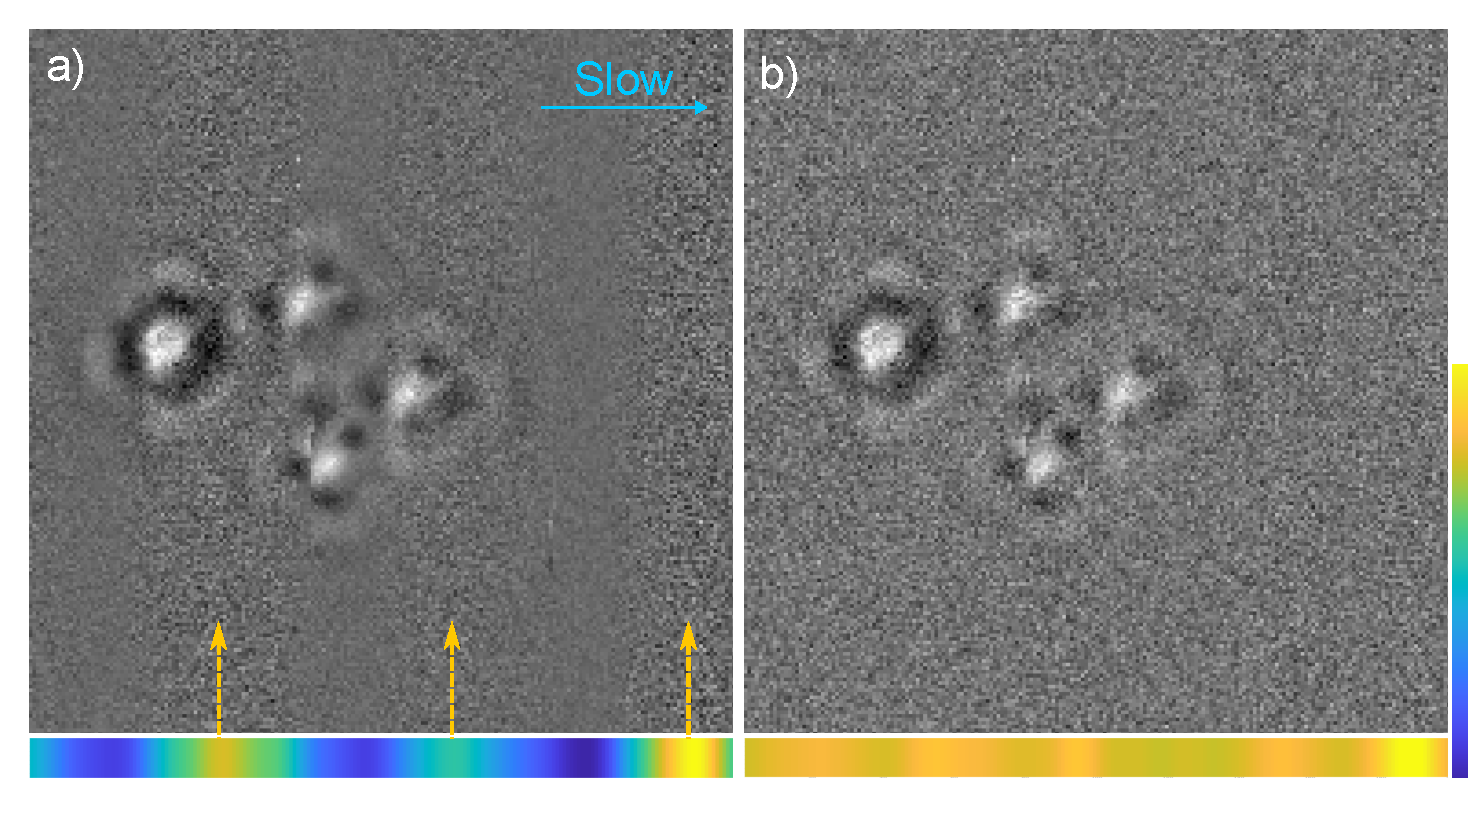
\includegraphics[width= \textwidth]{periodic_noise.pdf} 
	\centering
	\caption[\textbf{Leveling structured noise in PtSn$\textsubscript{4}$ grid spectroscopy data}]{\textbf{Leveling structured noise in PtSn$\textsubscript{4}$ grid spectroscopy data}. (a) Raw grid map collected over three days shows periodic noise patterns along the slow scan direction, with three distinct high–low noise cycles. (b) Noise-leveled data after variance matching across regions. The noise variation is shown in the color strip on the bottom of each image, with the yellow being high variation and blue being low variation.}
	\label{fig:periodic_noise}
\end{figure}

Lastly, an unstable \ac{STM} tip cause artifacts in grid spectroscopy measurements. A common  artifact is the streak noise, an artifact where a single or a few consecutive scan lines (usually along the fast scan direction) show a sudden deviation in signal current — due to transient disturbances during data acquisition. Often the streaky noise induced by tip change can be modeled as the intrinsic signal plus an offset. As illustrated in panel a) and b) in Figure. \ref{fig:streaks}, we can introduce streaks by applying a global offset on top of the signals in vertical lines (the fast scan direction). The global offset can be cured by leveling the means of data points on every column. An example is given in panel c) and d) in Figure. \ref{fig:streaks}, where the global streak removal algorithm successfully cured streaks with full vertical span. However, this algorithm is unable to resolve partial streaks, two examples are highlighted in the green box; we thus developed a method to identify and cure the partial streaks, with its detail expanded in the appendix.

\begin{figure}
	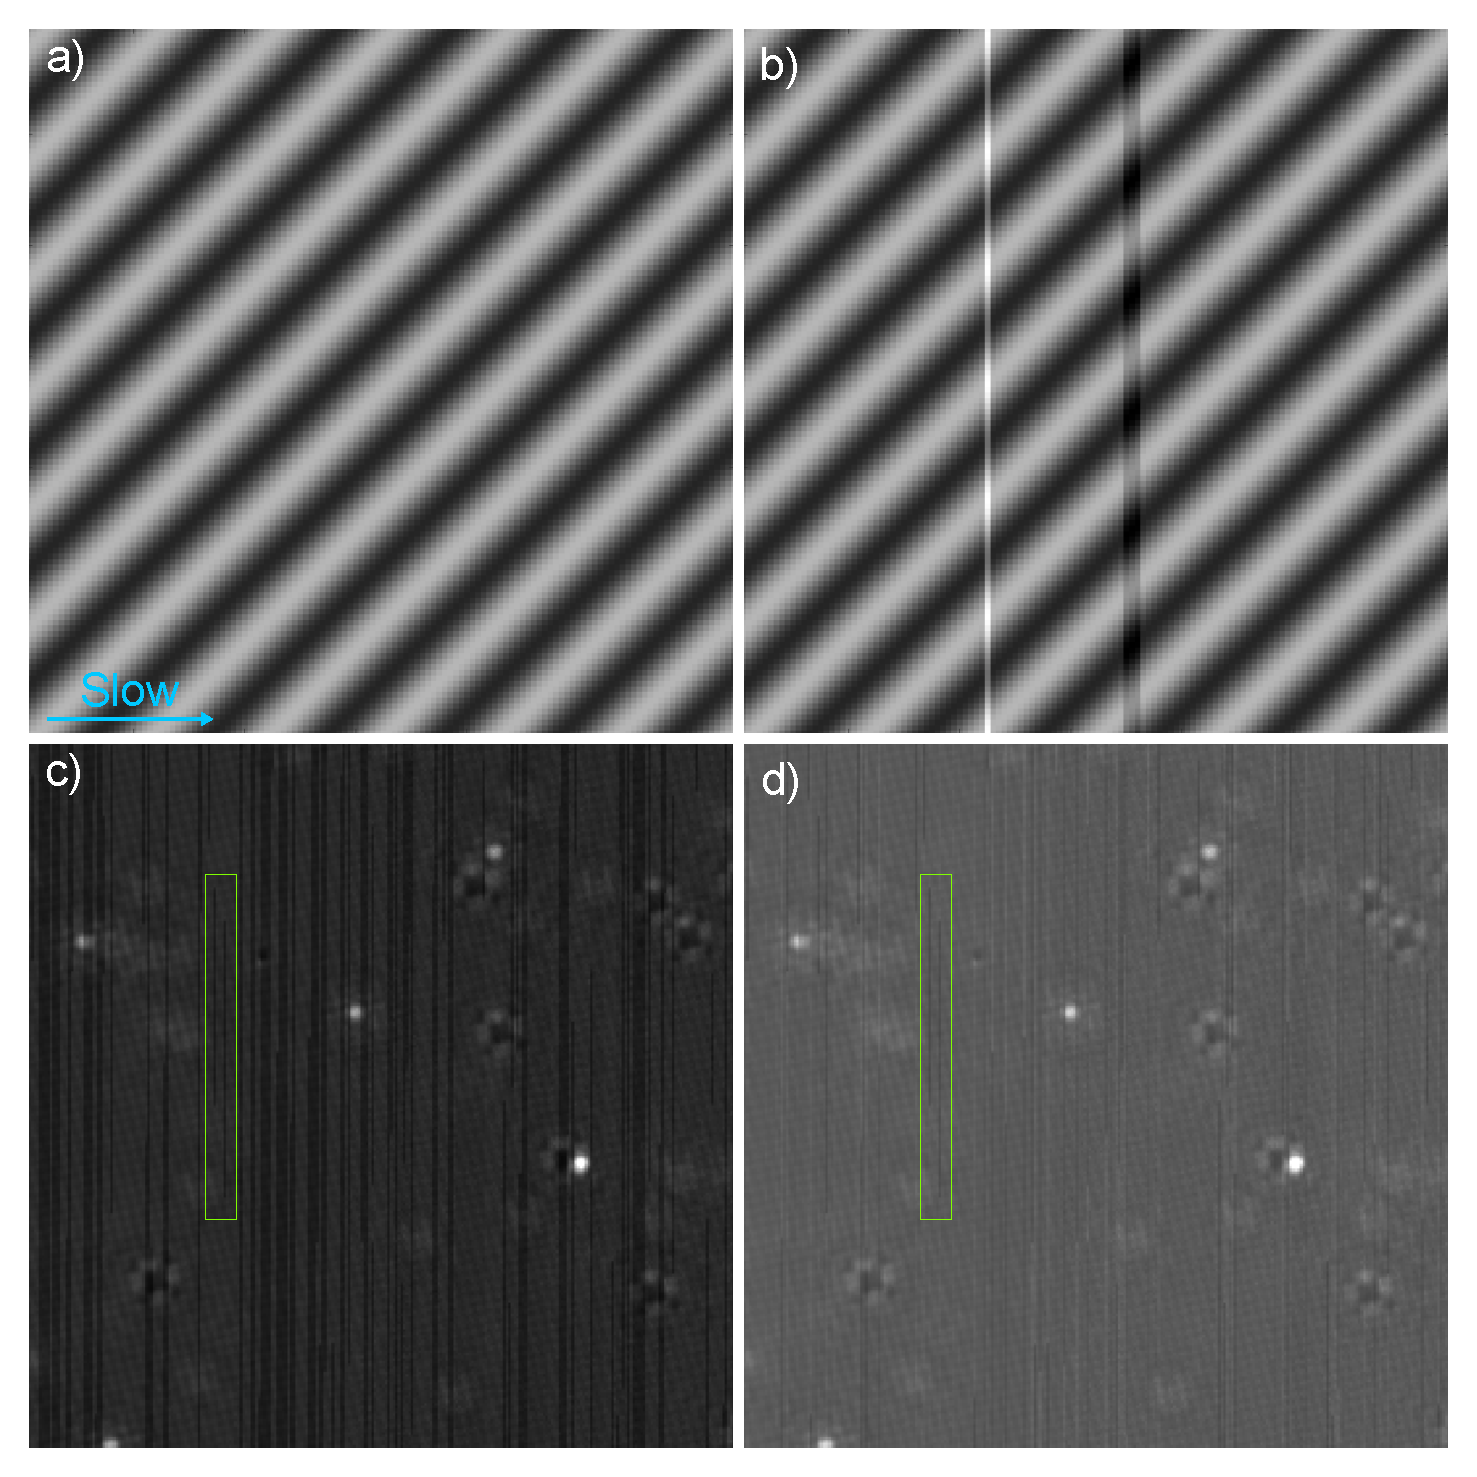
\includegraphics[width= \textwidth]{streaknoise.pdf} 
	\centering
	\caption{Streak noise illustration. a) simulated periodic data, with horizontal slow scan direction. b) streaked image, streaks are created by offsetting a column or several consecutive columns of signal. c): an illustration of the streak noise in real data. If we apply conventional global streak removal algorithm, we get d), however, there are still partial streaks that remain as highlighted in the green box.}
	\label{fig:streaks}
\end{figure}

\begin{figure}
	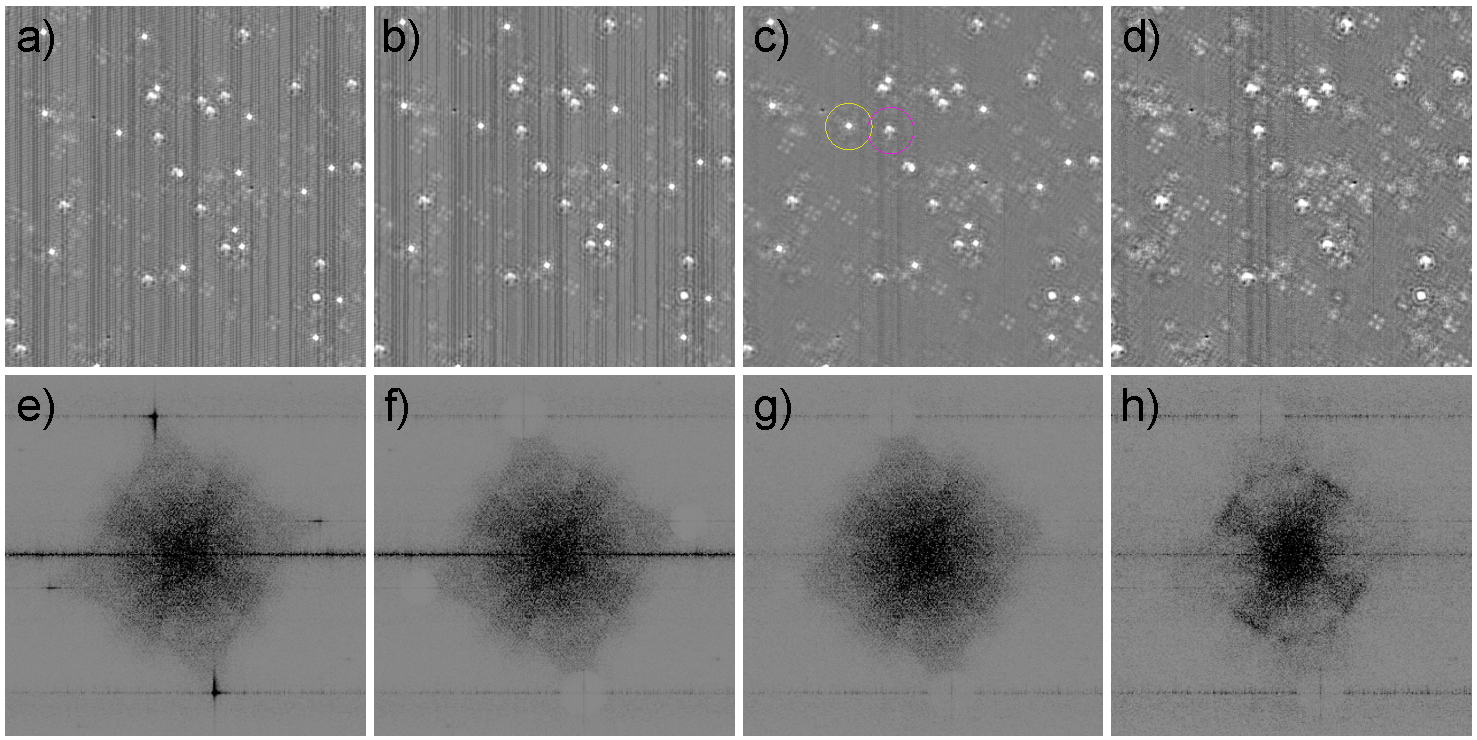
\includegraphics[width= \textwidth]{preprocessing_pipeline.pdf} 
	\centering
	\caption{Preprocessing pipeline for STM-QPI data illustrated using a ZrSiTe dataset. (a) Raw image showing strong horizontal streak noise, confirmed by the corresponding zero-frequency signal in the Fourier space (e). (b) Image after corrugation removal by masking the Bragg peaks in q-space. (c) Result after applying the streak removal algorithm, with improved clarity and reduced directional artifacts; corresponding Fourier transform g) shows suppression of the horizontal streak signal. (d) Image after masking the high-intensity yellow-type defects in c), using a truncated Gaussian mask with smooth tapering, revealing finer features in the remaining defect structures.}
	\label{fig:pipeline}
\end{figure}

Apart from the complexities and mitigation discussed above, there are other more standardized steps one usually takes in an STM-QPI analysis. We collected a series of operations and bundled them into a preprocessing pipeline; The raw data is fed into this pipeline and then the outcome will be fed into the algorithm. We illustrate this pipeline in Figure. \ref{fig:pipeline}. A raw ZrSiTe image is shown in a), we can see a large amount of streak noise, which causes the strong horizontal signal at zero frequency in the Fourier transform shown in e). We first remove the atomic corrugation by masking out the four Bragg peaks in the q-space as shown in f); this step is to ensure all the signal variation comes from the modified \ac{LDOS} from different impurities. We then apply the streak removal algorithm and get c); most streaks are removed, especially the more severe ones, leaving us with a cleaner dataset with only minor artifacts. This method's success can also be seen in q-space, where the horizontal DC signal is strongly suppressed; We can see from c) that there are multiple types of defects presented in this dataset, where examples of two most prominent types are circled in yellow and purple. It is also a good practice to mask out the defect centers to reduce the large intensity variations; in this case, we masked out the defect centers of the yellow type since its intensity is 10 fold that of the pristine area and 4 fold that of the purple type. The mask we used is a truncated Gaussian, which suppresses the signal locally around each defect center without introducing abrupt cutoffs. Its maximum value is capped at 0.99, ensuring that the defect signal is nearly removed while preserving surrounding features. To avoid artificial edges that could distort downstream analysis, I introduced a hyperbolic tangent–based step function that smoothly tapers the mask. After masking all occurrence of the yellow type defect, we are granted with image d) where the fine defect features are more clearly revealed. Now that we established the preprocessing pipeline, we are ready to apply the algorithm to some real datasets and present their results. 

\section{MC-SBD-STM results on experimental data}
In total, we applied the algorithm on 4 grid maps on 4 materials: Ag(111), LiFeAs, ZrSiTe and PtSn$_4$. For each dataset, we follow a two-stage process; first we apply the algorithm to a 2D single slice(aka the reference slice) of the grid map, we then take the output activation map from the single slice run as part of the initial guess, and apply the algorithm to a 3D block of the grid map. Note that both the amplitude of QPI patterns created by different defects and the noise level normally varies with energy. Since we can pick a reference slice that has strong QPI pattern and low noise level, the first stage is often less challenging. We can thus define a partial or complete success by whether the algorithm succeed on only the single slice or both the single slice and a block of the grid map. 

We will show below that the algorithm obtains a complete success on Ag(111) and ZrSiTe datasets, a partial success on LiFeAs dataset, and failed on the PtSn$_4$ dataset.  We will briefly introduce each systems we studied, and present their results in the following sections; all the technical details of the algorithm runs, including system parameters and initialization definition, will be included in the running files in the MC-SBD github repository under \textit{\slash examples}. 

\section{Ag(111)}

\begin{figure}
	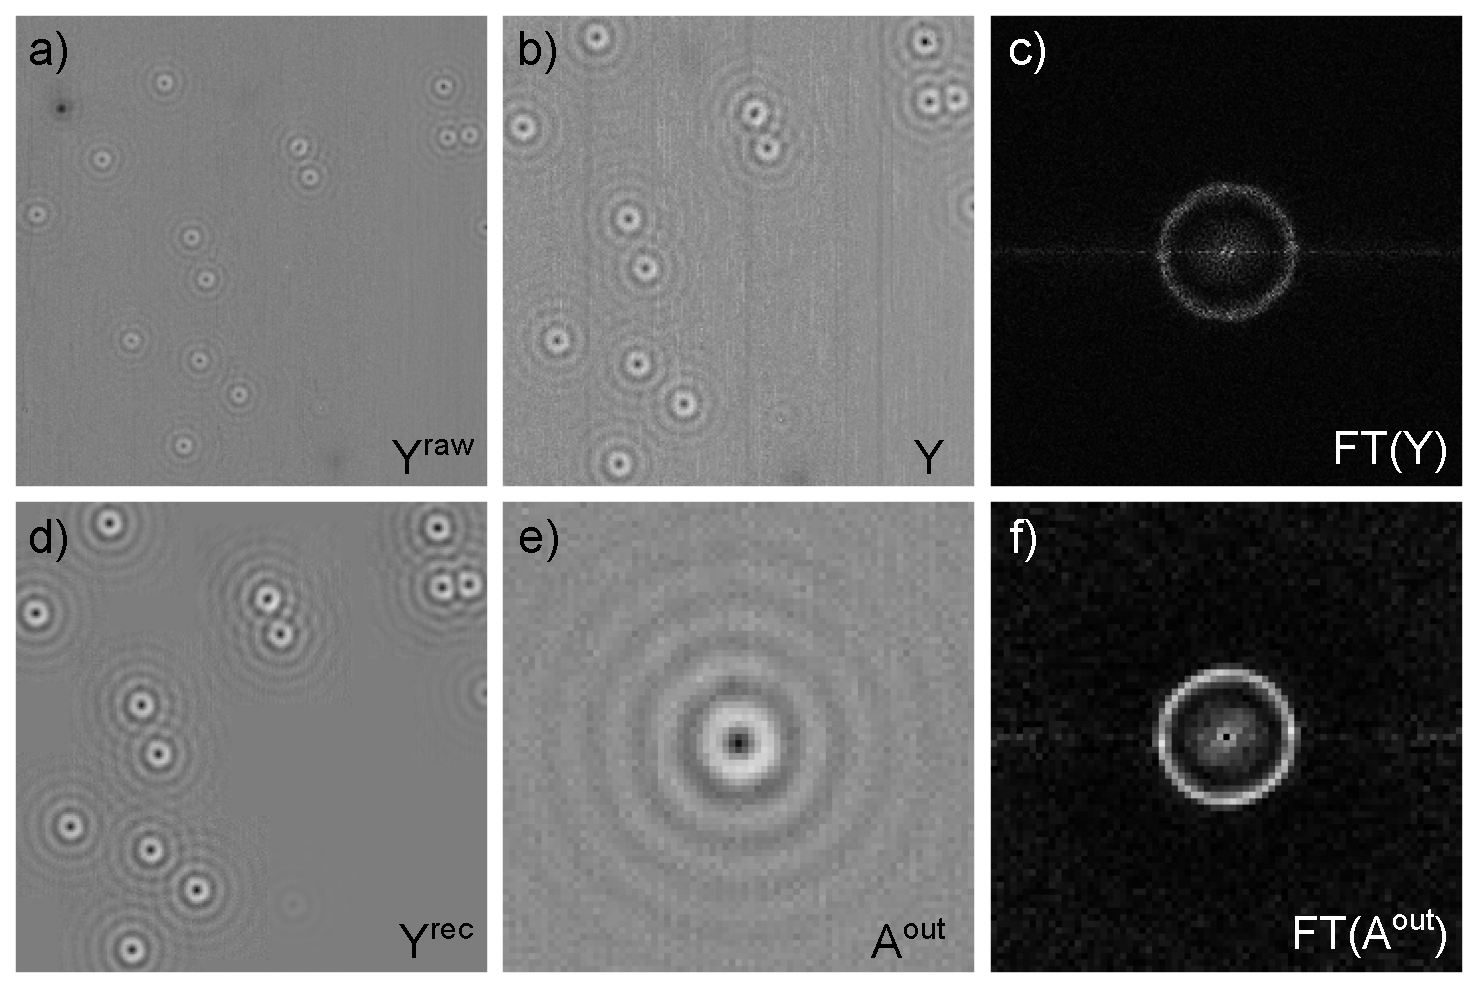
\includegraphics[width= \textwidth]{Ag1.pdf} 
	\centering
	\caption[\textbf{Application of MC-SBD algorithm to a single energy slice of an Ag(111) grid spectroscopy}]{\textbf{Application of MC-SBD algorithm to a single energy slice of an Ag(111) grid spectroscopy}. The raw dI/dV map at the Fermi level (a) shows QPI patterns around CO adsorbates. After cropping and streak removal, the processed observation $Y$ (b) serves as input to the algorithm. Its Fourier transform (c) reveals typical speckle noise that obscures fine momentum-space features. The algorithm reconstructs a speckle-free observation $Y^{rec}$ (d) using the learned output kernel (e) and activation map. The Fourier transform of the output kernel (f) reveals a clear, ring-like intra-band scattering signal, consistent with Ag(111)’s simple surface band. }
	\label{fig:Ag1}
\end{figure}

\begin{figure}
	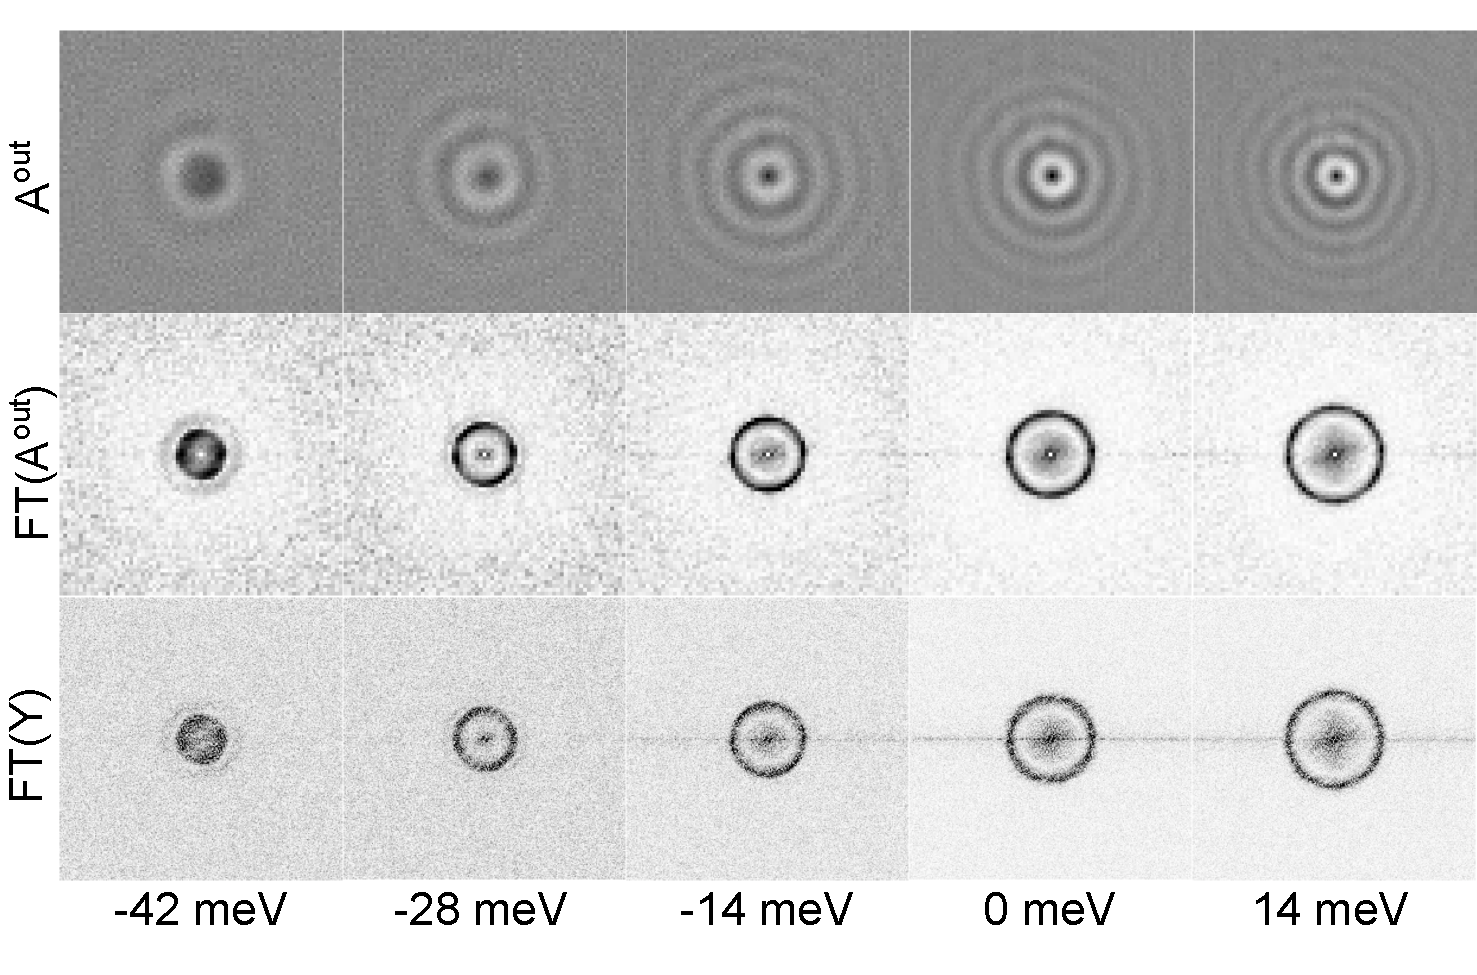
\includegraphics[width= \textwidth]{Ag2.pdf} 
	\centering
	\caption{\textbf{Energy-dependent reconstruction of QPI features in Ag(111) using MC-SBD-STM}. Five evenly spaced energy slices around the Fermi level are shown column-wise, revealing strong dispersion in the QPI pattern around CO molecules. The reconstructions in second row provide FT-QPI free from speckles, compared to the ones obtained directly from FT($Y$) as shown in row number three.}
	\label{fig:Ag2}
\end{figure}

Silver is a noble metal with a broad 5s conduction band crossing the Fermi level and a filled 4d manifold several eV below. In the bulk FCC Brillouin zone, these bands are separated near the L point, which is the center of the hexagonal surface along (111) direction. Thus when we project the bulk BZ along onto (111) surface, the band separation turns into a gap near the $\bar{\Gamma}$ point of the 2D BZ. This forms a so-called L-gap in Ag(111), and creates an energy window at $\bar{\Gamma}$ where no bulk-projected states exist. Within this window, a Shockley-type surface state forms\cite{bendounanEvolutionRashbaSpinorbitsplit2011}\cite{burgiQuantumCoherenceLifetimes2000}. It appears as a parabolic two-dimensional band with energy dispersion:
\begin{equation}
	E_{k} = E_0 + \frac{\hslash^2k^2}{2m^*}, 
\end{equation}
where $E_0 \approx 63$meV, and $m^*$ is the effective mass of the quasiparticle \cite{paniagoTemperatureDependenceShockleytype1995}. Because it resides entirely inside the L-gap, the surface state cannot hybridize with bulk states at small in-plane momentum and remains confined to the surface. This protection gives the Ag(111) surface state unusually long lifetimes and coherence, making it one of the cleanest systems for exploring quasiparticle interference and two-dimensional electron dynamics near the Fermi energy. 
 
To induce strong \ac{QPI} patterns, CO molecules can be deposited on Ag(111). A slice of the raw grid map at the Fermi level is shown in panel a) of the Figure. \ref{fig:Ag1}, which is featured by QPI pattern around CO adsorbates as impurities. We then process the raw image with cropping and streak removal to get the input observation $Y$ in b). The Fourier transform of the observation $Y$ shows a pattern of speckles. We then apply the \ac{MC-SBD} algorithm and get an output kernel $A^{out}$ as shown in e); together with the output activation map, we reconstructed an observation $Y^{rec}$ d) that successfully resembles the original observation $Y$. The q-space QPI map f), or the Fourier transform of $A^{out}$, is free from speckle as expected; the clear ring feature directly reflects the intra-band scattering of Ag's simple single band across the Fermi level. 

Impurity scattering by CO adsorbates on Ag(111) spans a wide energy range. We can thus apply the algorithm to the corresponding energy range of the grid map; out of the 120 slices, we show examples of the reconstructions near the Fermi level in the Figure. \ref{fig:Ag2}. It is worth noting that while running the algorithm on multiple slices, the activation map across different slices is identical for a single type of defect; since we get a perfect reconstruction on the slice at Fermi level(0 meV), results from other slices are guaranteed to be high-quality and thus trustworthy. This effectively constructs a 3D kernel across both spatial and energy dimensions, and allows us to access energy dispersion of QPI features free from speckles, which can be clearly illustrated by comparing the second and third rows of the Figure. \ref{fig:Ag2}.
\section{LiFeAs}

\begin{figure}
	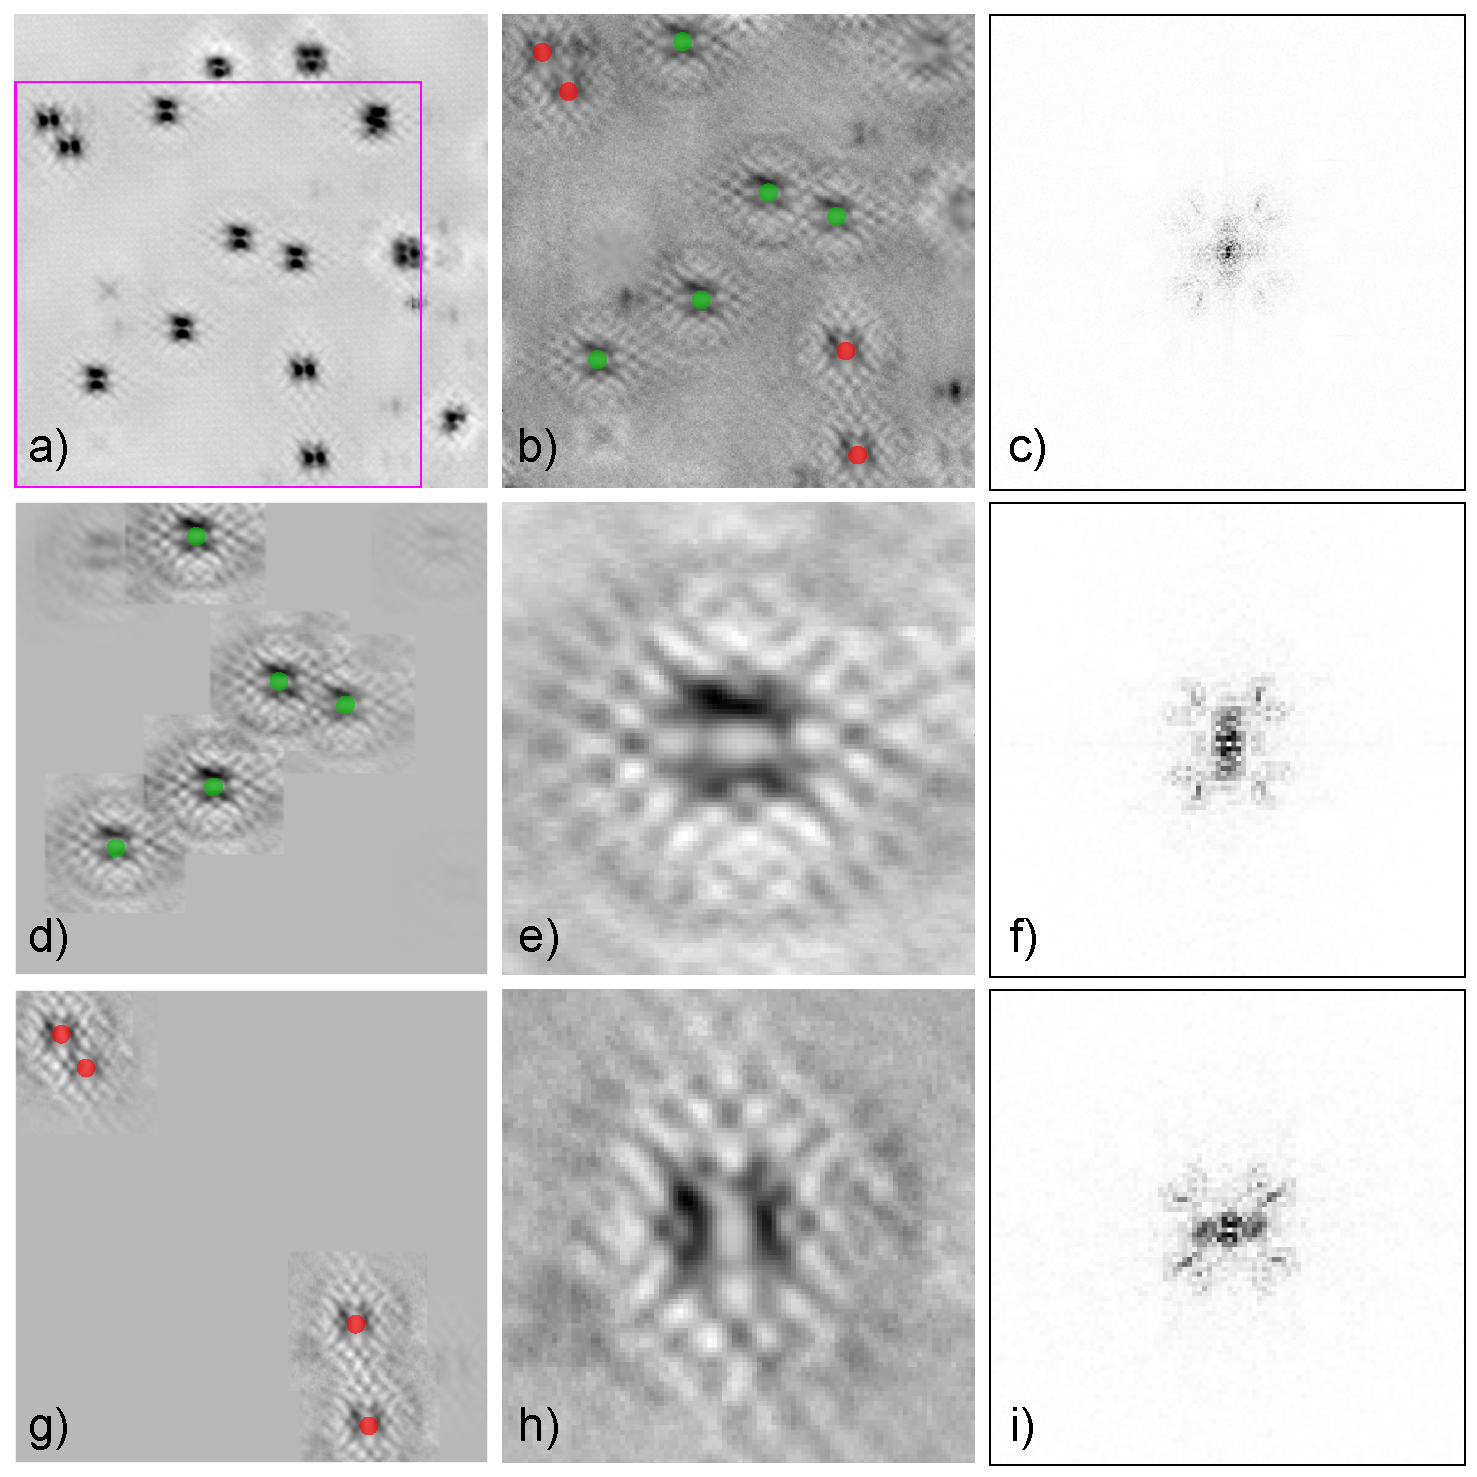
\includegraphics[width= \textwidth]{LiFeAs.pdf} 
	\centering
	\caption{Application of MC-SBD-STM to LiFeAs, a Fe-based superconductor with multiple impurity types. Panel a) shows the raw conductance slice near the Fermi level. In panel b), after preprocessing (cropping, streak removal, and defect center masking), red and green markers denote two orientations of a dominant defect type. Treating these as distinct kernels, the algorithm successfully demixes and reconstructs their contributions, as shown in d) and g), with marker overlays confirming accurate activation matching across both orientations. The output kernels are shown in e) and h), with the corresponding FT-QPI shown in f) and i).}
	\label{fig:LiFeAs}
\end{figure}
Fe-based unconventional superconductor LiFeAs hosts diverse and rich scattering signatures; the associated \ac{QPI} patterns encode information about both the underlying band structure and the superconducting order parameter. A notable example is the \ac{QPI} study by Chi et al.\cite{chiSignInversionSuperconducting2014}, which exploited the real-space interference pattern to extract phase-sensitive information on the superconducting gap structure and provided strong evidence for $s_{\pm}$ pairing. However, their analysis required cropping the real-space QPI image around selected defects, a step that inevitably risks contamination from neighboring scatterers and complicates the interpretation of subtle phase features. The algorithm we present offers a potential pathway to overcome this limitation: by reconstructing single-defect kernels directly, it can isolate the QPI of individual scatterers and thus provide a cleaner window into the phase structure of unconventional superconductors.

Panel a) in Figure. \ref{fig:LiFeAs} is a slice of the grid spectroscopy on LiFeAs near the Fermi level. Among multiple types of impurities presented, there is a type of impurity with two different orientations that dominates in numbers. This can be better seen in b), an image that undergoes the processing of cropping, streak removal, and defect center masking. In b), red and green markers are manually labeled on the defect centers of the horizontal and vertical orientations, respectively. Despite being the same type of defect, the algorithm treats these two orientations as two types of kernels. We thus choose the number of kernels to be two, and apply the algorithm to the observation in b). We then get two output kernels, e) and h), and the reconstructed observations, d) and g). The markers in d) and g) are copied from b) as references to the defect locations. We can clearly see that the reconstructed observations successfully identified all occurrences of the defect in both orientations. This illustrates the algorithm's ability to both demix and deconvolute the experimental grid spectroscopy(single slice) into multiple kernels and their activation locations. 

It is worth noting that the algorithm mistakenly treats the defect on the top right corner as an occurrence of a horizontally oriented kernel; however, the influence from this assignment is minimal due to its faint activation. This run of the algorithm gives us an observation fidelity of ~0.5, half of the ideal $\textbf{\textit{OF}} =1$. This might be counter-intuitive as we did see a nearly perfect identification of the activation for both kernels; this discrepancy roots from the fact that apart from the 2 kernels the algorithm reconstructs, there are intensities from other types of defects contributing to the original observation. For instance, the 'X'-shaped defect on the bottom left corner will remain in the residual observation $Y^{res} = Y - \sum_i Y_i^{rec}$; this is actually desirable since the contribution of other defect types is not used to deconvolute the designated kernels, making the reconstruction more trustworthy. Therefore, in cases where the observation consists of defect types other than the reconstructed kernels, we need both \textbf{\textit{OF}} and the empirical observation of the activation matching to assess the quality of reconstruction.  

This example illustrates that our approach can disentangle the QPI signatures of individual defect types from the background of other scatterers. In doing so, it helps to mitigate the broader limitations faced by defect-specific real-space analyses—which often rely on cropped regions and thus risk contamination from neighboring scatterers.
\section{ZrSiTe}
\begin{figure}
	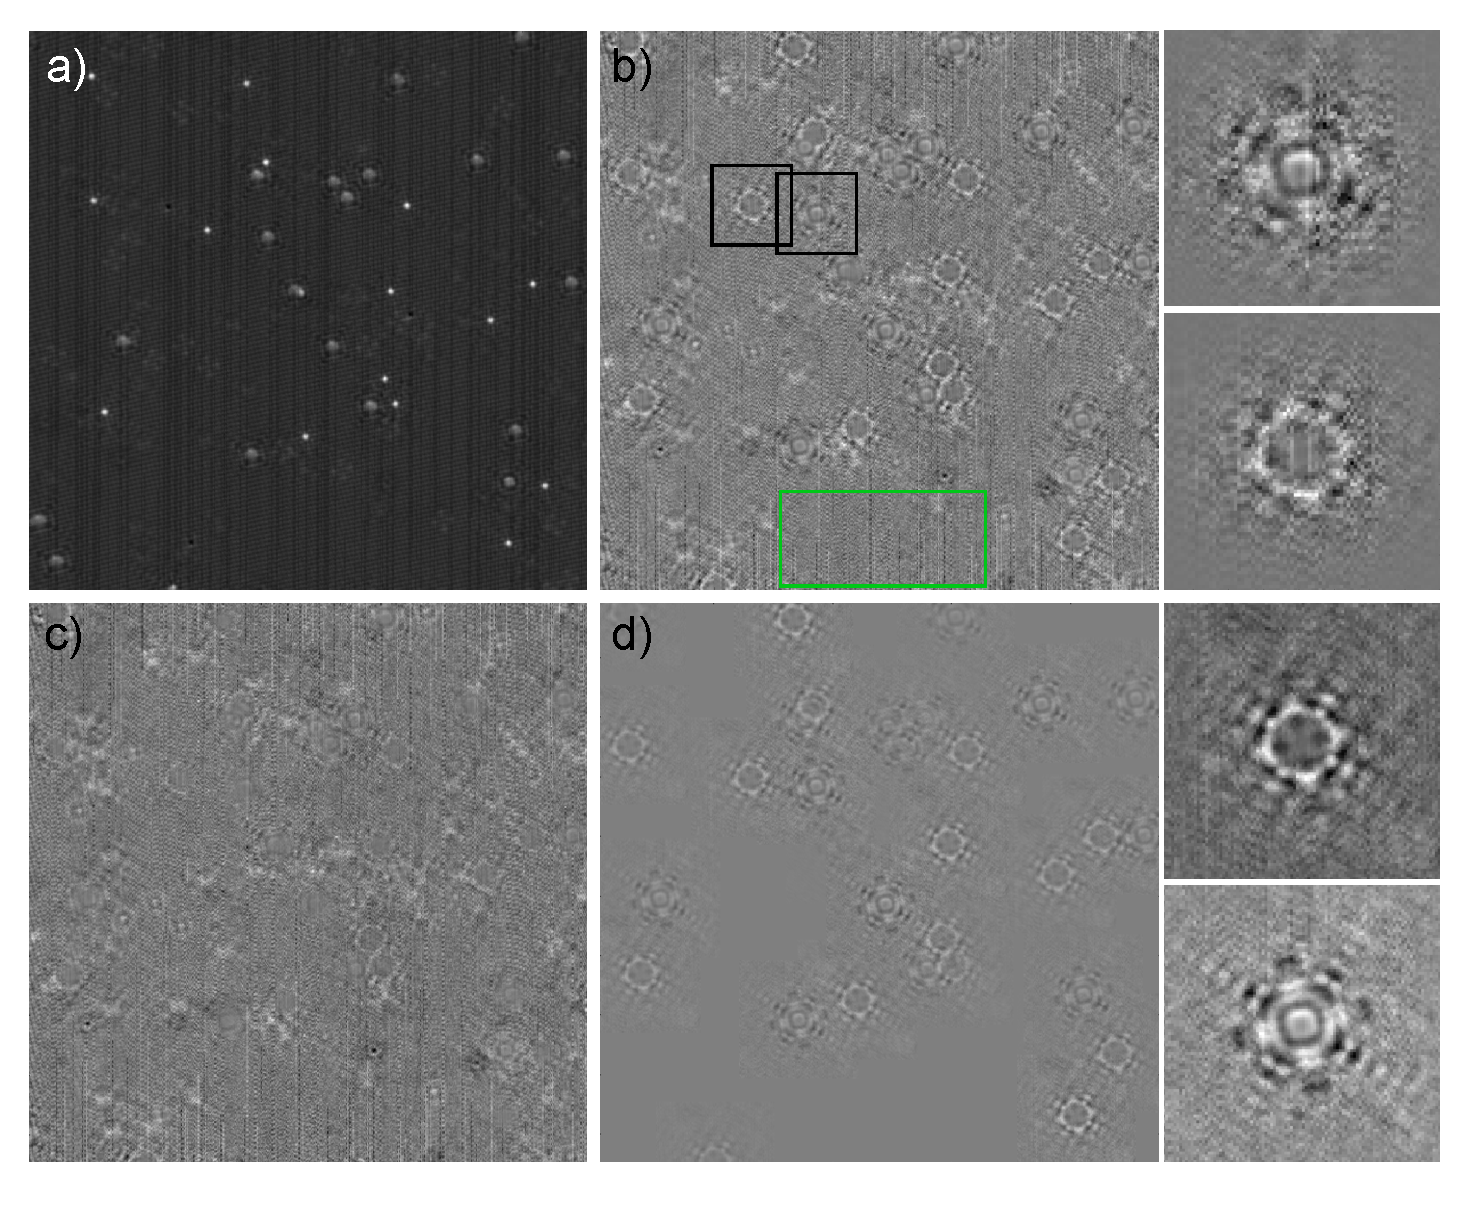
\includegraphics[width= \textwidth]{ZrSiTe1.pdf} 
	\centering
	\caption[\textbf{Overview of MC-SBD-STM applied to ZrSiTe}]{\textbf{Overview of MC-SBD-STM applied to ZrSiTe}. Panel a) shows a reference slice (E = -168 meV) of the grid map; b) is the preprocessed observation $Y$ after Bragg peak masking, cropping, streak removal, and defect center masking. Two kernel initializations are extracted from the black boxes in b), Gaussian-windowed and shown to the right. The reconstructed observation (d) closely resembles b), while the residual (c) captures streak noise and unmodeled features. Despite the presence of residuals, the observation fidelity (OF) is 1.1 due to the dominance of structured noise in both residual and background regions.}
	\label{fig:ZrSiTe1}
\end{figure}
\subsection{Introduction}
Quasiparticle interference (QPI) has proven to be a powerful tool to probe the electronic topology of the ZrSiX (X=S, Se, Te) family of Dirac nodal-line semimetals. The space group P4/nmm of this family exhibits nonsymmorphic symmetry, and results in floating band surface states. These surface states have significant influence on the electronic properties, and serve as major scattering channels in \ac{QPI} measurements, as found in both ZrSiS\cite{butlerQuasiparticleInterferenceZrSiS2017} \cite{lodgeObservationEffectivePseudospin2017} and ZrSiSe\cite{toppSurfaceFloating2D2017}\cite{zhuQuasiparticleInterferenceNonsymmorphic2018}\cite{buVisualizationElectronicTopology2018}. In contrast, the case of ZrSiTe presented a puzzle: while QPI measurements captured many expected band-derived features, the floating-band scattering remained conspicuously absent \cite{stuartQuasiparticleInterferenceObservation2022}. Studies also found that this family hosts multiple types of impurities, with some couple differently to the band structure, and producing distinct scattering characteristics\cite{butlerQuasiparticleInterferenceZrSiS2017}\cite{stuartQuasiparticleInterferenceObservation2022}. The presence of multiple defects with defect-specific scattering features makes the ZrSiX a test field for our algorithm. 

In this section, we revisit ZrSiTe with our algorithm; it successfully disentangle defect-specific scattering both from individual slices and from a block of data spans a wide energy range. The output not only resolves high-quality distinct \ac{QPI} patterns for different defects, but also provides tantalizing evidence of features consistent with the elusive floating-band scattering predicted by theory, suggesting that what was once deemed “mysteriously missing” in ZrSiTe may now be within reach.

\subsection{Result}
Figure. \ref{fig:ZrSiTe1} shows an overview of the application of the algorithm. The input observation b) is the post-processed image from raw data a); it underwent the process of Bragg peak removal, cropping, streak removal, and defect masking. We run the algorithm with two initialized kernels shown on the right of b); the initial guesses are cropped from the two black boxes in b) with a Gaussian window($\sigma = 3$) applied to damp the features on the edges. Panel d) shows the reconstructed observation, with two output kernels shown on the right. This reconstruction gives a residual observation $Y^{res}$ shown in c), on which most of the streaky noise and contributions from other defects are left. We then look at \textbf{\textit{OF}}, the variance ratio between the noise region (see the green box in panel b)) and the residual observation. The resulting \textbf{\textit{OF}} is 1.1, which might be surprising, as we have contributions from other defects in the residual observation. The reason is that most of the intensity variations are actually from the streaky noise; since the reconstructed observation d) is free from streaks, the same level of streaks is presented in both the noise region and the residual observation. 

We thus take a closer look at the activation match between the reconstructed and original observations. As shown in Figure. \ref{fig:ZrSiTe2}, we first annotate all occurrences of both defect types in circle markers as shown in c), then overlay these markers to defect-specific reconstructed observations a) and b); the perfect activation match indicates a high reconstruction quality. We can also note that the occurrence number is 16 for defect type 1, and 17 for defect type 2; these numbers are close to the critical occurrence threshold $N^{critical}$ for $SNR=1$ according to the Figure. \ref{fig:KS_vs_N}. Given the $SNR$ of our system exceeding 1, we should expect a perfect reconstruction from the output kernels.

The output kernels in panels d) and e) show two different QPI patterns. We can better characterize the difference between the two scattering features in q-space; in panel f), the QPI signal features two concentric squares, and these two squares are also nested with their sides in parallel. QPI signal in panel g) is substantially different; it features an inner square and a circle that are concentric. Moreover, there are also two sets of parallel lines in the radial directions that stick out from the outer circle. These distinct scattering signatures are inaccessible from h), the direct Fourier transform of the observation, in which defect-dependent scattering features are entangled.

\begin{figure}
	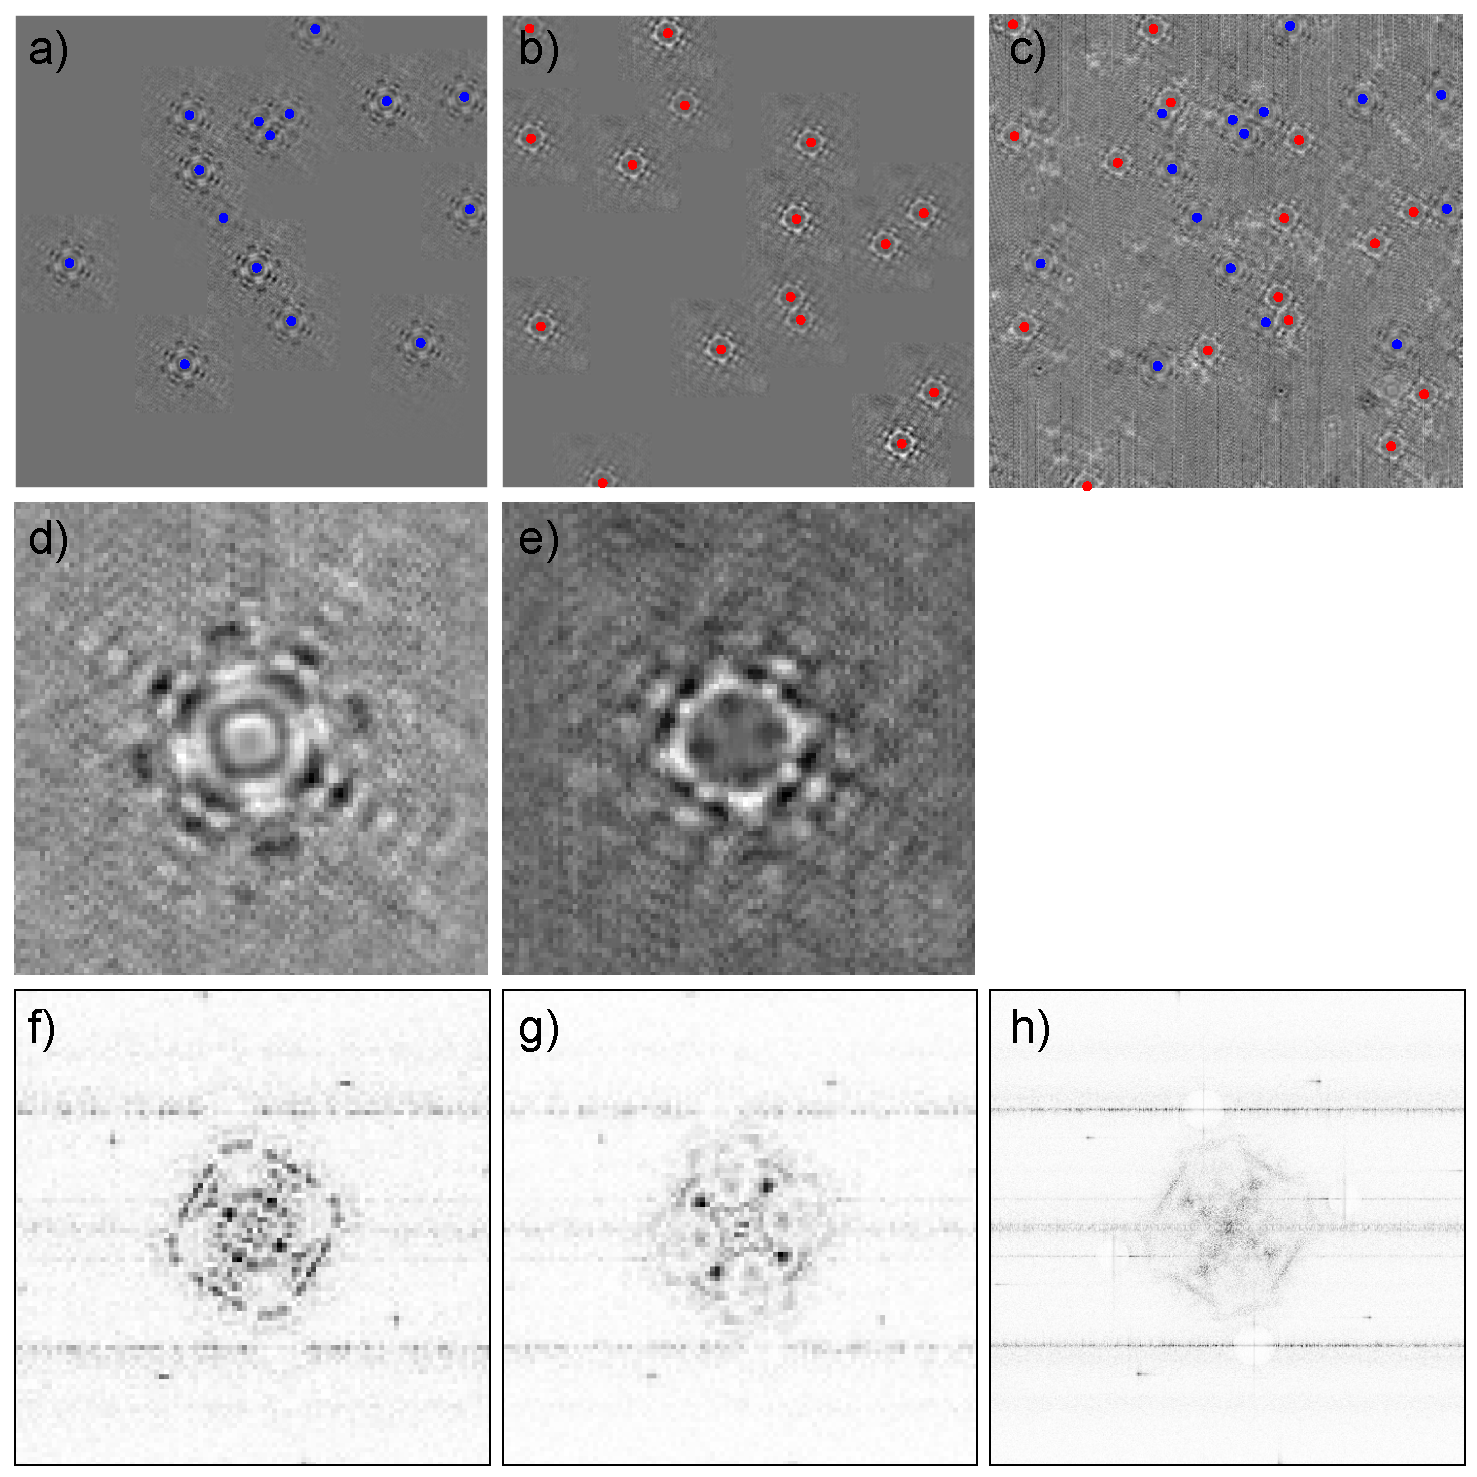
\includegraphics[width= \textwidth]{ZrSiTe2.pdf} 
	\centering
	\caption[\textbf{Validation of the activation match in ZrSiTe}]{\textbf{Validation of the activation match in ZrSiTe}. Panels a) and b) display the defect-specific reconstructed observations, with overlayed markers indicating true defect locations annotated in c). The one-to-one match between reconstructions and true activations confirms high reconstruction quality. Panels d) and e) show the output kernels for the two defect types. Their corresponding QPI patterns in q-space (f, g) exhibit distinct geometries, such as concentric squares and circular features, which are entangled in the conventional FT-QPI shown in h).}
	\label{fig:ZrSiTe2}
\end{figure}

We further apply the algorithm to the whole block of the grid. We are able to get the energy-dependent defect-specific scattering features for both types across a full bias range of -800 meV to 800 meV, with an energy resolution of 8 meV. As an example, we plot 5 evenly spaced energy slices of the two output kernels around the Fermi level in Figure. \ref{fig:ZrSiTe3}. We can make a simple observation of the second and fourth row, and find that the q-space QPI patterns for both defects are highly dispersive in energy; this indicates that both defects indeed contribute, but in different ways, to the electron-impurity scattering in ZrSiTe. Studying these impurity-dependent dispersive features can help us uncover the underlying scattering mechanism behind each impurity type and further expand our understanding of this system. 

Defect states present themselves differently in different energy levels. In ZrSiTe, when bias exceeds 200 meV, an additional type of defect becomes equally prominent compared to the two types mentioned above, and we can run the algorithm with an additional number of kernels on slices beyond $E=200meV$. The result of an example slice at $E=320meV$ is shown in the Figure. \ref{fig:ZrSiTe4}. The algorithm successfully ran with four kernels, with reconstructed observation b) that closely resembles the original observation a). Panel c)-d) are output kernels for the two known defect types, whereas e)-f) are the output kernels of two orientations for this new type of defect that looks like the symbol 'H'.  

\begin{figure}
	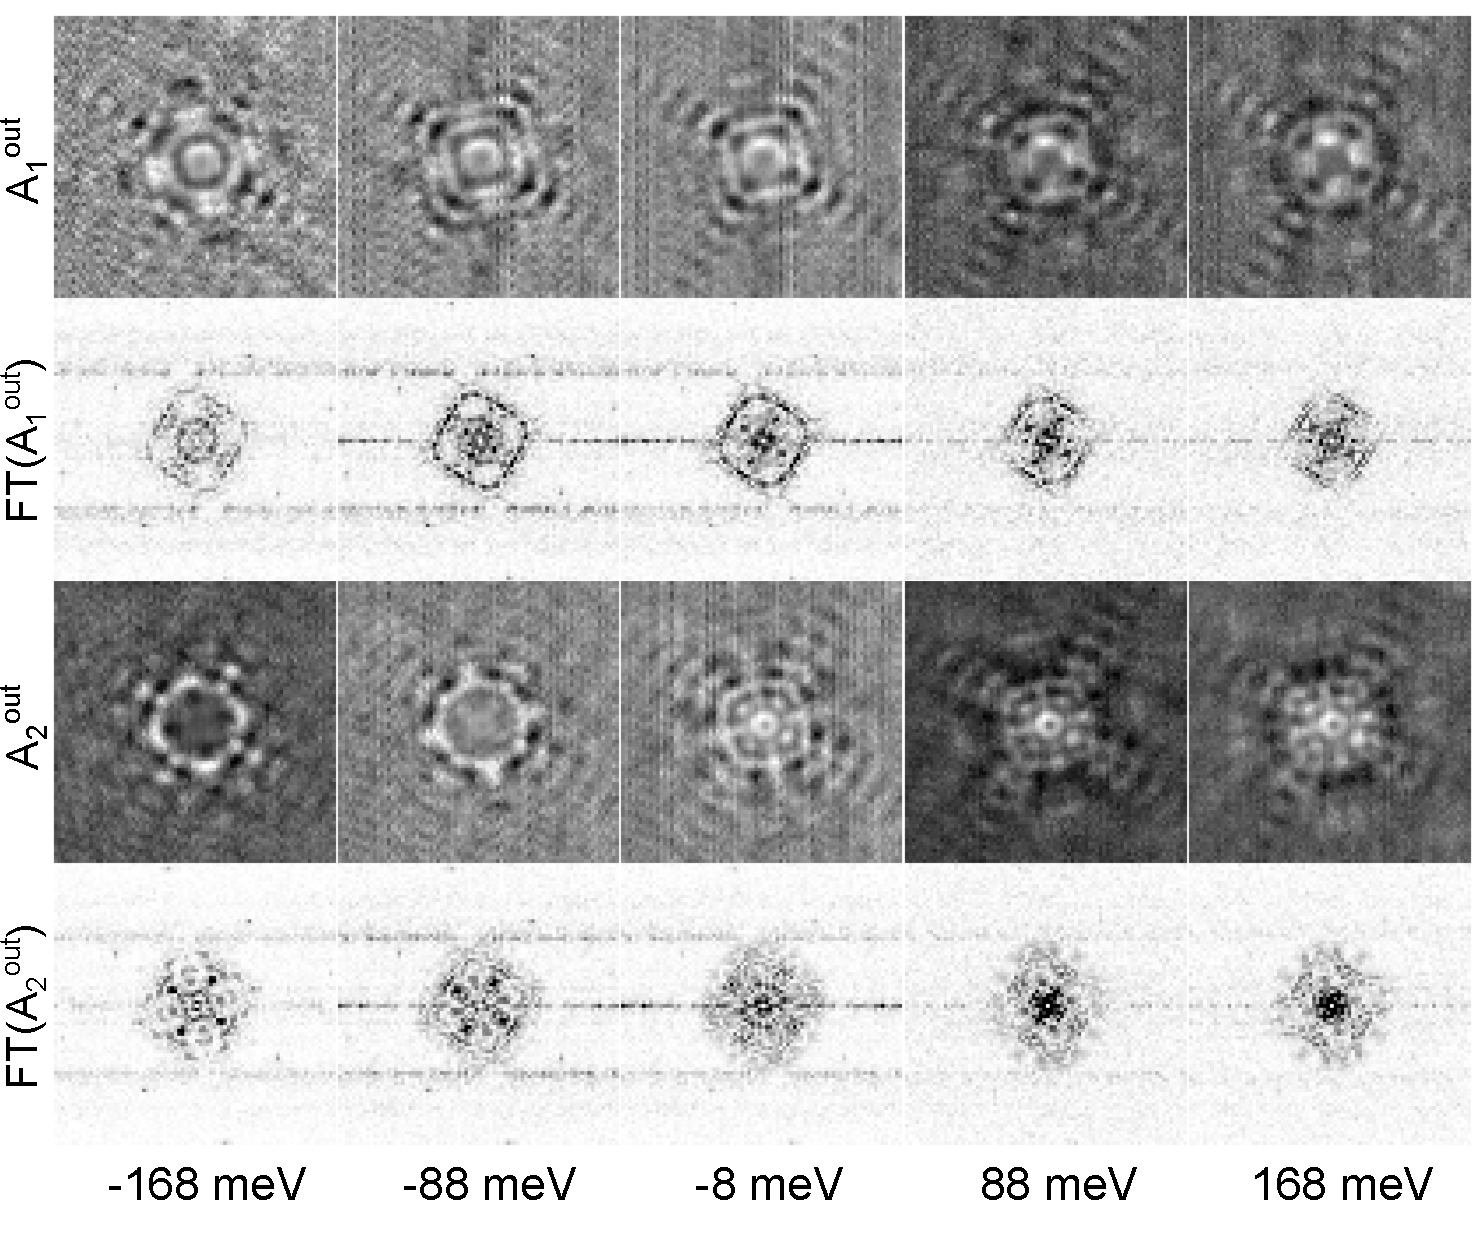
\includegraphics[width= \textwidth]{ZrSiTe3.pdf} 
	\centering
	\caption[\textbf{Energy-dependent reconstruction of defect-dependent scattering in ZrSiTe using MC-SBD-STM}]{\textbf{Energy-dependent reconstruction of defect-dependent scattering in ZrSiTe using MC-SBD-STM}. Five evenly spaced energy slices around the Fermi level reveal strong dispersion in the QPI patterns of both defect types. This confirms that both types contribute differently to the scattering across energy, enabling energy-resolved analysis of defect-specific scattering processes in ZrSiTe.}
	\label{fig:ZrSiTe3}
\end{figure}

\subsection{Signature of floating band scattering}
TO BE WRITTEN

To conclude, the algorithm run on the ZrSiTe dataset illustrates that given proper preprocessing on real datasets with a sufficient number of defect occurrence, the \ac{MC-SBD} algorithm is capable of delivering high-quality reconstruction up to 4 kernels across a wide range of energy.

\begin{figure}
	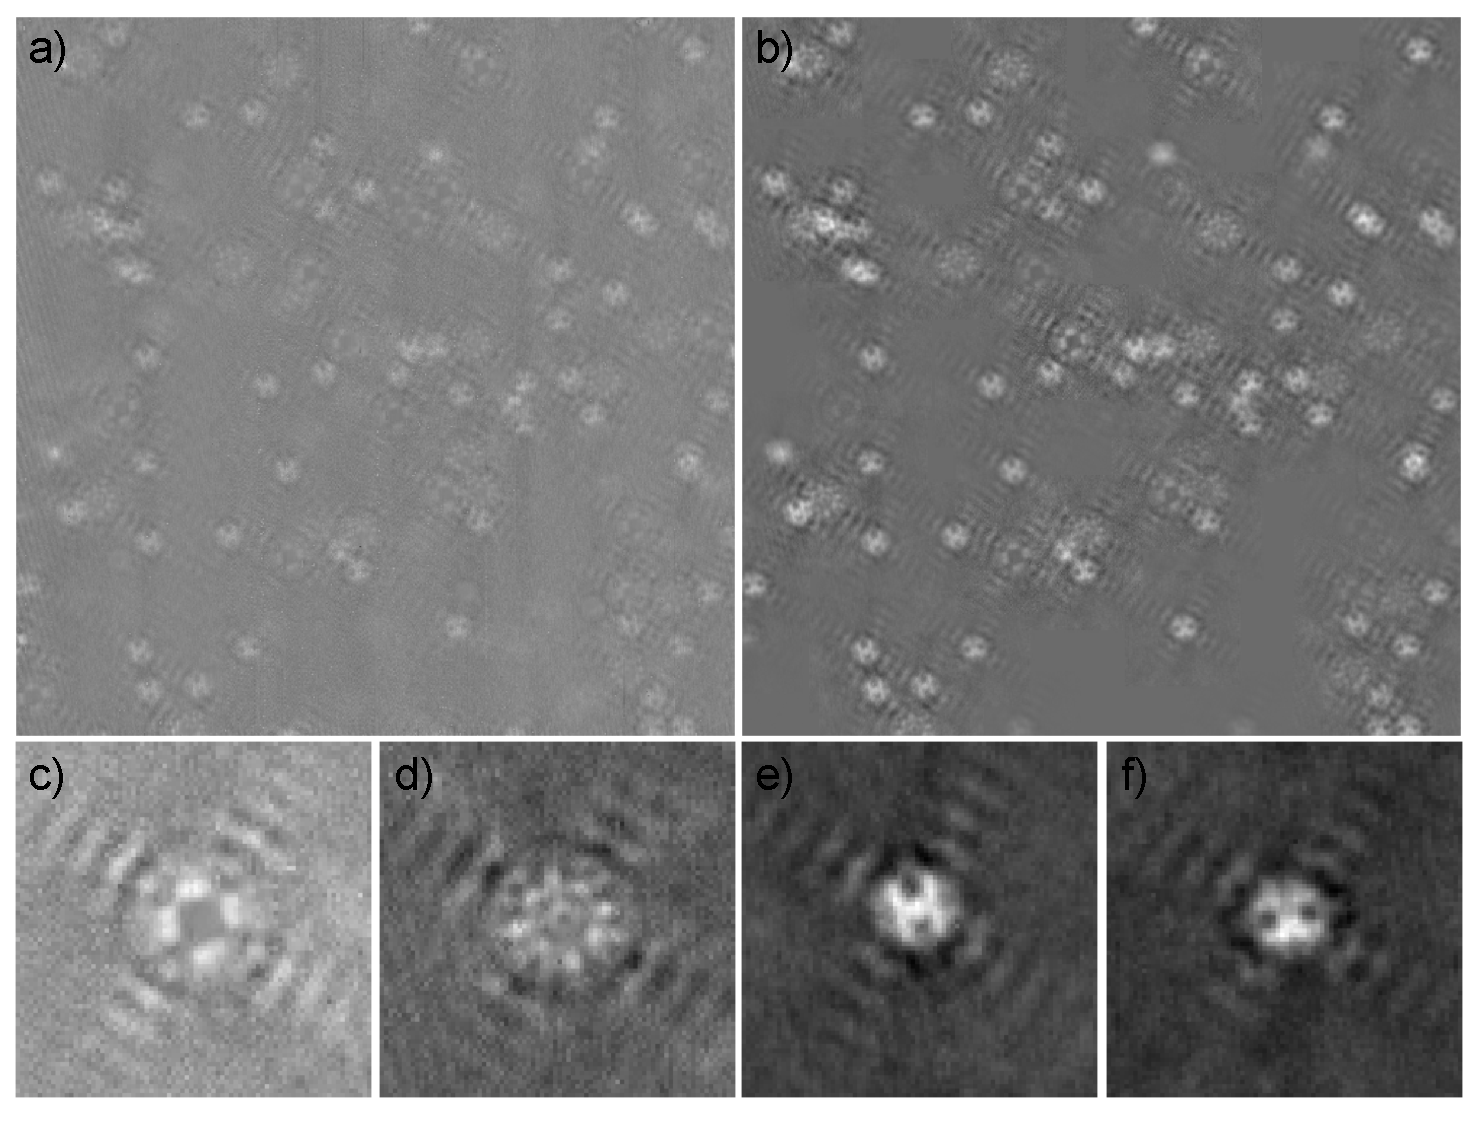
\includegraphics[width= \textwidth]{ZrSiTe4.pdf} 
	\centering
	\caption[\textbf{Four-kernel reconstruction at 320 meV in ZrSiTe}]{\textbf{Four-kernel reconstruction at 320 meV in ZrSiTe}. A new defect type becomes prominent at this energy. The original and reconstructed observations (a, b) closely match. Output kernels for the known defect types are shown in c) and d), while the two orientations of the new, H-shaped defect are captured in e) and f). This demonstrates the algorithm’s capability to resolve multiple distinct scattering channels when sufficient occurrences are available.}
	\label{fig:ZrSiTe4}
\end{figure}

\section{PtSn\textsubscript{4}}

PtSn\textsubscript{4} exhibits a set of properties that make it inherently challenging for algorithmic deconvolution. First, as shown in section \ref{section:defect_spectro}, point spectroscopy shows that individual defects have only a limited impact on the local electronic structure, giving rise to \ac{QPI} patterns of low intensity. In addition, the defect density across the sample is very low, and the Sn-site defects can occur in multiple orientations, further reducing the effective occurrence number available for statistical averaging. Taken together, the combination of weak scattering, sparse defect populations, and orientation multiplicity creates an intrinsically adverse dataset. These unfavorable conditions render the system a natural stress test for the algorithm, probing its robustness under particularly stringent limits of signal and statistics.

We applied the algorithm to a dataset of PtSn\textsubscript{4}, with the topographic image and the raw grid map slice shown in panels a) and b) of Figure \ref{fig:PtSn4}, respectively. To increase the chance of a successful run, the reference slice in panel b) was selected for its strongest QPI pattern within the entire grid map. We prepared two observations with identical preprocessing, except that $Y_1$ in panel c) omits noise leveling, while $Y_2$ in panel d) includes it. The noise leveling procedure referenced here was previously illustrated in Figure \ref{fig:periodic_noise}.

We performed two algorithm runs on $Y_1$, using both four and two kernel types. The initial guesses for both runs are indicated by the black boxes in panel c), with two additional green boxes added for the four-kernel case. A separate two-kernel attempt was performed on $Y_2$, with initializations marked by yellow boxes in panel d). The resulting reconstructed observations, output kernels, and residual observations from these three attempts are shown in panels e)–f), g)–h), and i)–j), respectively. To state the conclusion upfront: all three attempts failed, but in different ways. By examining the reasons behind each type of failure, we can gain deeper insights into the algorithm's limitations and identify strategies to improve data acquisition.

First, from the topography shown in panel a), we observe two types of defects. The second type, identified as the $Sn\textsubscript{3}$ defect (see Figure \ref{fig:ch4_defectgallery} panel c), appears in three distinct orientations. The raw observation $Y_{\text{raw}}$ clearly shows that the QPI patterns differ across these orientations. Based on this, we employed four kernel types in Attempt 1. However, each kernel type is represented by only a single occurrence, which eliminates the algorithm’s denoising capability. In addition, demixing fails due to significant overlap between the spatial regions associated with each defect. With only one occurrence per kernel, any intensity in the overlapping regions can be arbitrarily distributed among kernels without altering the data fidelity term, introducing infinite degeneracy. In other words, the output remains unchanged even if one kernel “steals” intensity from another in the overlap region, representing a worst-case scenario of linear mixing equivalence(a review can be found in section 5.2.1).

Further issues can be seen in the reconstructed observation (panel e), where the algorithm incorrectly identifies two noise patches along the right edge as valid activations—likely a result of structured noise in the input $Y_1$. Lastly, although this run yields an observation fidelity of \textbf{\textit{OF}} = 1.06, it serves as a reminder that \textbf{\textit{OF}} alone is not always a reliable indicator of reconstruction quality.

Recognizing that the primary limitation in Attempt 1 was the single occurrence per kernel, we reduced the number of kernel types to two in Attempt 2. While the defect centers in $Y_{\text{raw}}$ appear different, their associated QPI patterns away from the center may be similar across orientations. After masking the defect centers in both $Y_1$ and $Y_2$, it becomes plausible to treat the three orientations of the $Sn\textsubscript{3}$ defect as three instances of a single kernel. This adjustment leads to a noticeable improvement in reconstruction quality. The reconstructed observation (panel g) shows good agreement with all three activations of the $Sn\textsubscript{3}$ defect, and the observation fidelity improves to \textbf{\textit{OF}} = 1.21.

However, the reliability of this reconstruction remains questionable for two reasons. First, we lack validation for the critical assumption that QPI patterns from distinct defect orientations are identical. Second, the dataset has a relatively low signal-to-noise ratio ($SNR\sim 1$), and as shown in Figure \ref{fig:KS_vs_N}, a reliable reconstruction at this SNR level requires approximately 15 occurrences per defect type. Therefore, even if the assumption holds, the reconstruction may still be statistically unreliable.

Finally, the attempt using the post-noise-leveled dataset $Y_2$ also failed. Specifically, the output activation map for the $Sn\textsubscript{3}$ defect (panel i) poorly matches the expected defect locations. Since Attempts 2 and 3 share identical parameters and initializations, this outcome demonstrates that when the SNR is already low, the cost of increasing the overall noise level through noise-leveling can outweigh its benefits. In such cases, this preprocessing step may degrade rather than improve algorithm performance, and should be omitted.

\begin{figure}
	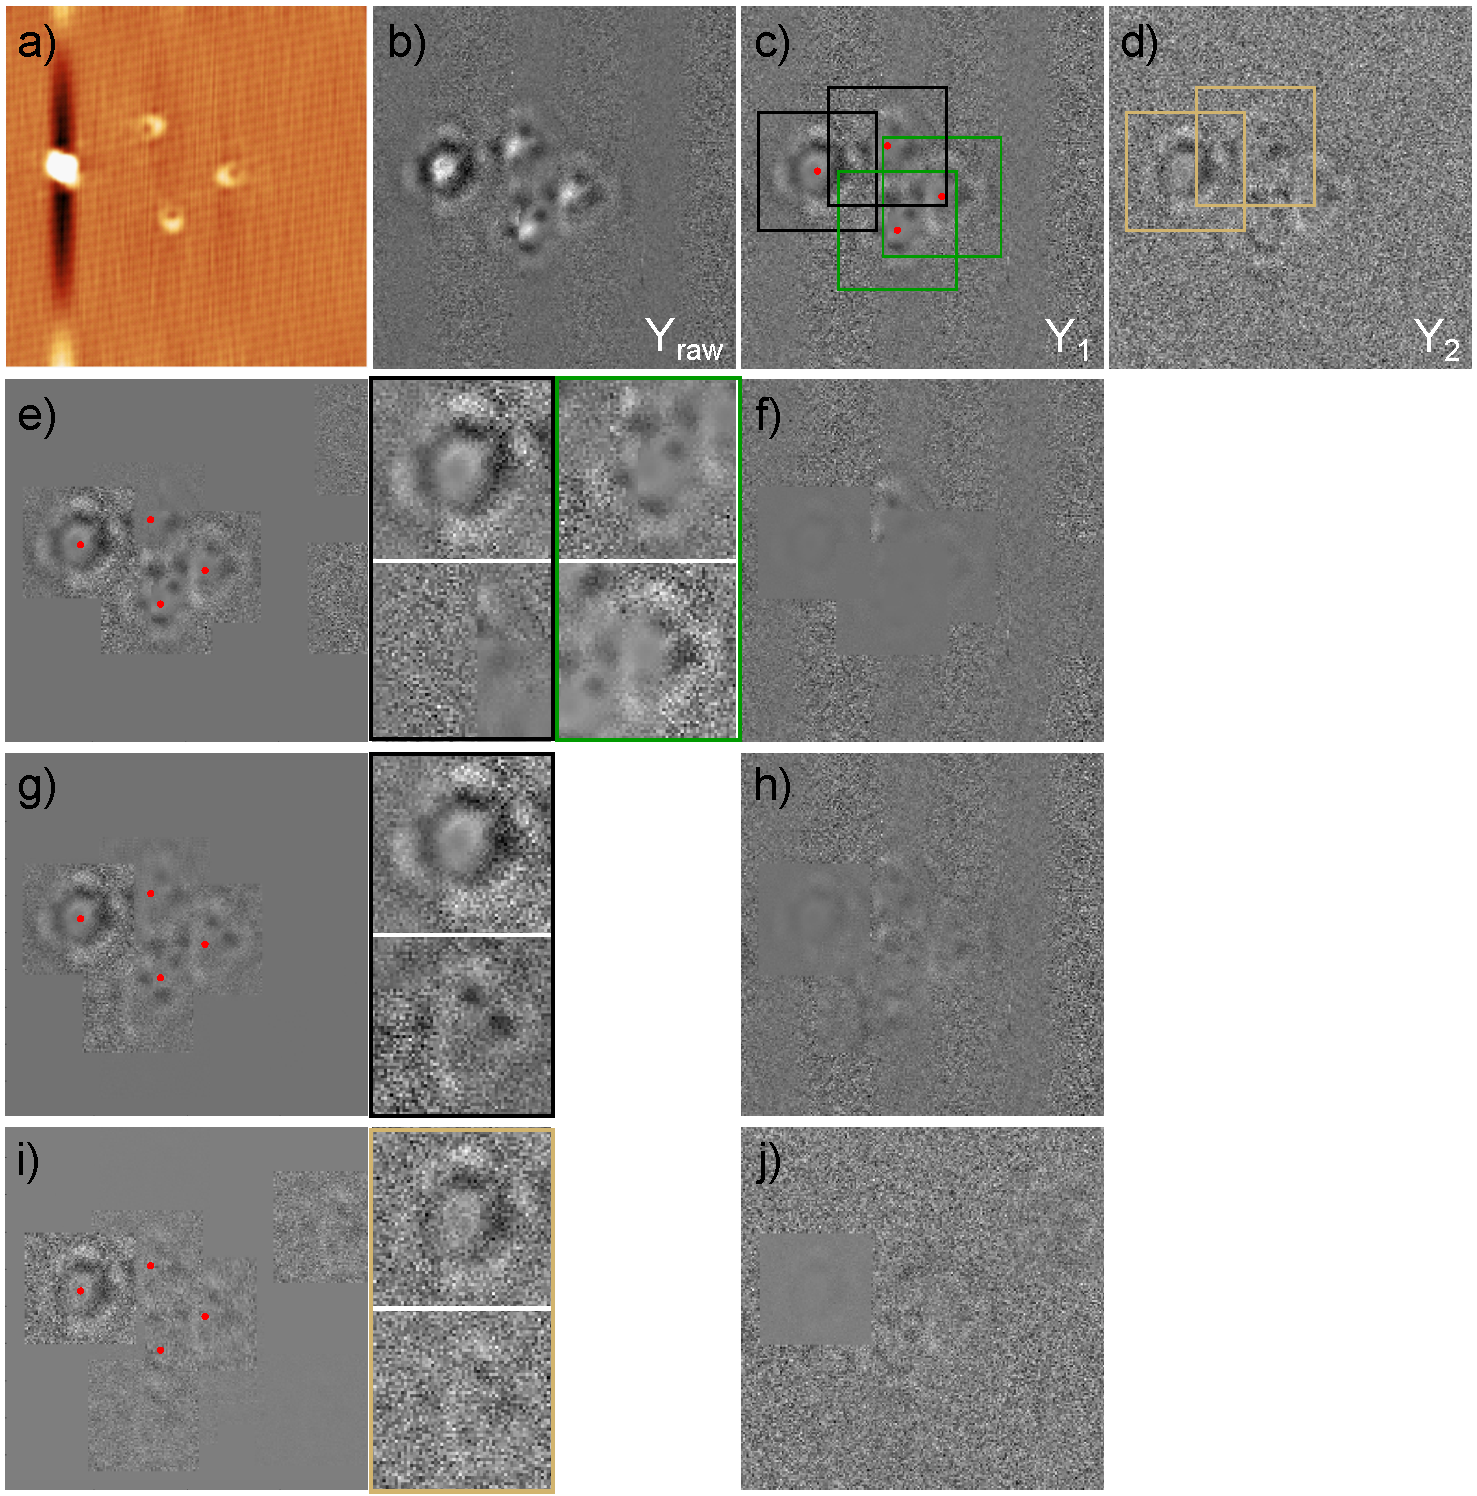
\includegraphics[width= \textwidth]{PtSn4_result.pdf} 
	\centering
	\caption[\textbf{Application of the MC-SBD-STM algorithm to a PtSn\textsubscript{4} dataset and analysis of failure modes}]{\textbf{Application of the MC-SBD-STM algorithm to a PtSn\textsubscript{4} dataset and analysis of failure modes}. (a) Topographic image and (b) raw grid spectroscopy slice showing QPI patterns from two defect types, including the three-orientation $Sn\textsubscript{3}$ defect. Two observations were prepared with identical preprocessing except for noise leveling: $Y_1$ without (c), and $Y_2$ with noise leveling (d), as illustrated in Figure \ref{fig:periodic_noise}. Initial kernel guesses for each attempt are marked: black and green boxes in (c) for the four- and two-kernel runs on $Y_1$, and yellow boxes in (d) for the two-kernel run on $Y_2$. Reconstructed observations (e–f), output kernels (g–h), and residuals (i–j) from the three attempts shows different level of failure. The red dots in the reconstructed observations are the ground truth defect locations from c)}
	\label{fig:PtSn4}
\end{figure}

\section{A practical guide to perform MC-SBD on real data}
This section summarizes key insights from the chapter and offers a set of practical guidelines to improve the success rate of applying the algorithm to experimental data.

Although we do not elaborate in detail on best practices for scanning tunneling spectroscopy (STS), it is important to emphasize that the algorithm’s success depends critically on acquiring high-quality grid maps. This involves shaping a stable tip, minimizing vibrational and electronic noise, and maintaining optimal system tuning throughout the measurement. These foundational practices should always be followed. In addition, particular attention must be paid to avoiding structured noise, which can severely degrade algorithm performance.

For optimal results, the grid map should ideally cover a region where the number of occurrences for each defect type of interest exceeds a threshold value, denoted as $N^{\text{critical}}$. Because defect types often vary significantly in their densities, it may be challenging to identify regions where all defect types are sufficiently represented. In such cases, it is advisable to focus on the defect types of greatest interest and select regions where these specific types surpass their respective $N^{\text{critical}}$.

The value of $N^{\text{critical}}$ depends on the signal-to-noise ratio (SNR) of the measurement, which can be estimated by comparing the contrast strength of the QPI pattern around a defect relative to the pristine background. The estimated $N^{\text{critical}}$ based on the SNR is given in the Figure. \ref{fig:KS_vs_N}, which was established in the synthetic data environment. However, due to additional complexities in experimental data, $N^{\text{critical}}$ is shown in Figure. \ref{fig:KS_vs_N} is often underestimated. To mitigate this, it is beneficial to include a larger number of defects by either (i) identifying regions with higher local defect density, or (ii) increasing the physical coverage of the grid. The latter option may be constrained by cryogenic holding time; one possible trade-off is to reduce the real-space resolution. However, as shown in Figures \ref{fig:phase_space} and \ref{fig:phase_spaceN=3}, excessively high local defect density (e.g., $\geq$ 0.1 defects per lattice site) leads to reconstruction failure, so regions with defect clustering should be avoided.

The algorithm allows users to specify the number of kernels and their sizes to deconvolve. The number of kernels should generally match the number of distinct QPI patterns corresponding to the defect types of interest; note that in the case of the same defect with different in-plane rotations, they are considered to have distinct QPI patterns, and we should use multiple kernels. Unrelated defect types can be ignored, as demonstrated in our analyses of LiFeAs (Figure \ref{fig:LiFeAs}) and ZrSiTe (Figure \ref{fig:ZrSiTe1}), where we used two kernels. However, if unwanted defects exhibit strong contrast, they can interfere with the reconstruction. In such cases, we recommend suppressing their signal intensity using truncated Gaussian masks during the preprocessing stage. When choosing kernel sizes, there are two considerations. First, recall the larger kernel sizes will increase the degeneracy space and poses a harder problem for the algorithm, as we discussed in Section 5.2.1, and shown in \ref{fig:ch6_t&s}; and the smallest kernel size should be big enough to cover the whole distinct QPI pattern in the observation $Y$, with the kernel edge being where the QPI signal amplitude meets the noise level. Second, due to the denoising capacity of the algorithm, the output kernel has a lower noise level and could uncover QPI features further from the defect center that was originally inaccessible from the observation $Y$; this sets the upper bound of the kernel size, with which we could retrieve more information in real space and better resolution in momentum space. The user is therefore recommended to start from the smallest and incrementally increase the kernel size until the algorithm fails to produce high-quality outputs. In terms of the kernel shape, while all the kernels used in this chapter are square, the algorithm allows for rectangular kernels, which could be useful for scattering features with spatial anisotropy.

As described earlier, the algorithm is typically run first on a single energy slice (“slice run”), followed by a full energy stack (“block run”) once success has been achieved on the slice. The block run benefits from the output activation maps of the slice run, which can be used as an initial guess. Since defect activations are assumed constant across energy, this initialization is often close to the global minimum of the data fidelity term and significantly improves the block run’s success rate.

Finally, note that the sparsity regularization parameter $\lambda_i^{\text{block}}$ for each kernel type $i$ should be scaled relative to the number of energy slices. Specifically, if the slice run used a value of $\lambda_i^{\text{slice}}$, then the block run with $N_{slices}$ slices should use:
\begin{equation}
	\lambda_i^{\text{block}} = \sqrt{N_{slices}}\lambda_i^{\text{slice}}
\end{equation}
A detailed discussion of the sparsity regularizar $\lambda$ can be reviewed in Section 5.3.2. 

\section{Summary and outlooks}
In this chapter, we presented a comprehensive validation and application of the MC-SBD-STM algorithm, showcasing its ability to demix, deconvolve, denoise, and ultimately extract defect-specific quasiparticle interference (QPI) patterns from both synthetic and experimental scanning tunneling microscopy (STM) data.

We first developed a simulation framework that addressed key limitations in prior synthetic QPI datasets. By grounding kernel truncation in signal-to-noise ratio (SNR) and enforcing lattice-consistent defect placements, we generated realistic test cases for benchmarking. To evaluate algorithm performance, we introduced four metrics—Kernel Similarity (KS), Activation Similarity (AS), Observation Fidelity (OF), and Demixing Score (DS). These enabled a systematic assessment of reconstruction quality across a broad parameter space. Our benchmarks revealed two key dependencies: kernel quality improves with the number of defect occurrences (due to denoising through averaging), while activation fidelity breaks down at high defect densities (due to increased interference). These observations led to the definition of a critical occurrence threshold, $N^{\text{critical}}$, providing a concrete guideline for experimental design. 

We then turned to the application of \ac{MC-SBD} to real STM datasets on four materials: Ag(111), LiFeAs, ZrSiTe, and PtSn\textsubscript{4}. To bridge the gap between simulation and experiment, we developed a preprocessing pipeline to mitigate real-world complexities, including streak noise, periodic environmental noise, and high-contrast defect centers. This standardization step was crucial for algorithm success on experimental data. The algorithm achieved full success on the Ag(111) and ZrSiTe datasets, producing clean, defect-resolved QPI patterns across energy. A partial success was observed in LiFeAs, where the dominant defect types were correctly identified and reconstructed, although the presence of other types reduced the overall observation fidelity. The run on PtSn\textsubscript{4} failed, due to insufficient defect statistics and unresolved experimental artifacts, reaffirming the practical importance of the guidelines established from synthetic benchmarks.

On the note of future studies, our algorithm can be leveraged to explore exotic scattering processes in emerging quantum materials. For example, in ZrSiTe – a nodal-line semimetal where conventional FT-QPI is dominated by a topological drumhead surface state, obscuring the “floating band” scattering observed in its sister compounds \cite{stuartQuasiparticleInterferenceObservation2022}\cite{butlerQuasiparticleInterferenceZrSiS2017}. One of the potential cause is that only one or a few types of defects couples to the "floating band", making its contribution in the FT-QPI obscure. Thus, having access to defect-specific scattering features is crucial to reveal these missing QPI features in momentum space.

On the other hand, by resolving interference from individual defects directly in real space, our approach preserves phase information that is lost in traditional Fourier-based analysis. This opens the door to phase-sensitive studies of scattering in materials like unconventional superconductors. For instance, one could identify Bogoliubov quasiparticle interference patterns governed by selection rules reflecting sign-reversed order parameters, information previously inaccessible via standard QPI techniques \cite{chiSignInversionSuperconducting2014}.